\subsubsection{Package sequenziatore::client::iview::iuser}

\paragraph{IMainUser}
\begin{figure}[H] \centering 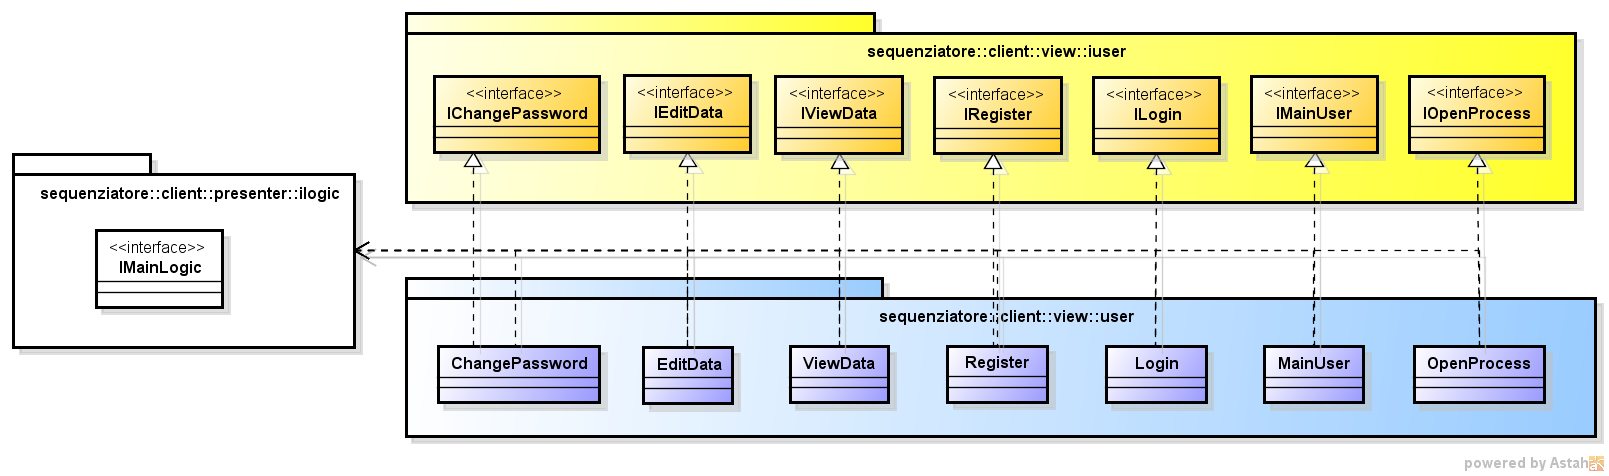
\includegraphics[width=%
\textwidth]
{./pack/viewuser.png} \caption{Diagramma comunicazione tra view e presenter}
\end{figure}
\begin{itemize}
\item \textbf{Nome:} \texttt{IMainUser};
\item \textbf{Package:} \texttt{\iViewUser{}};
\item \textbf{Descrizione:} Interfaccia che permette la gestione delle principali componenti dell'Interfaccia grafica dell'utente.
\end{itemize}

\paragraph{IUpdateView}
\begin{figure}[H] \centering 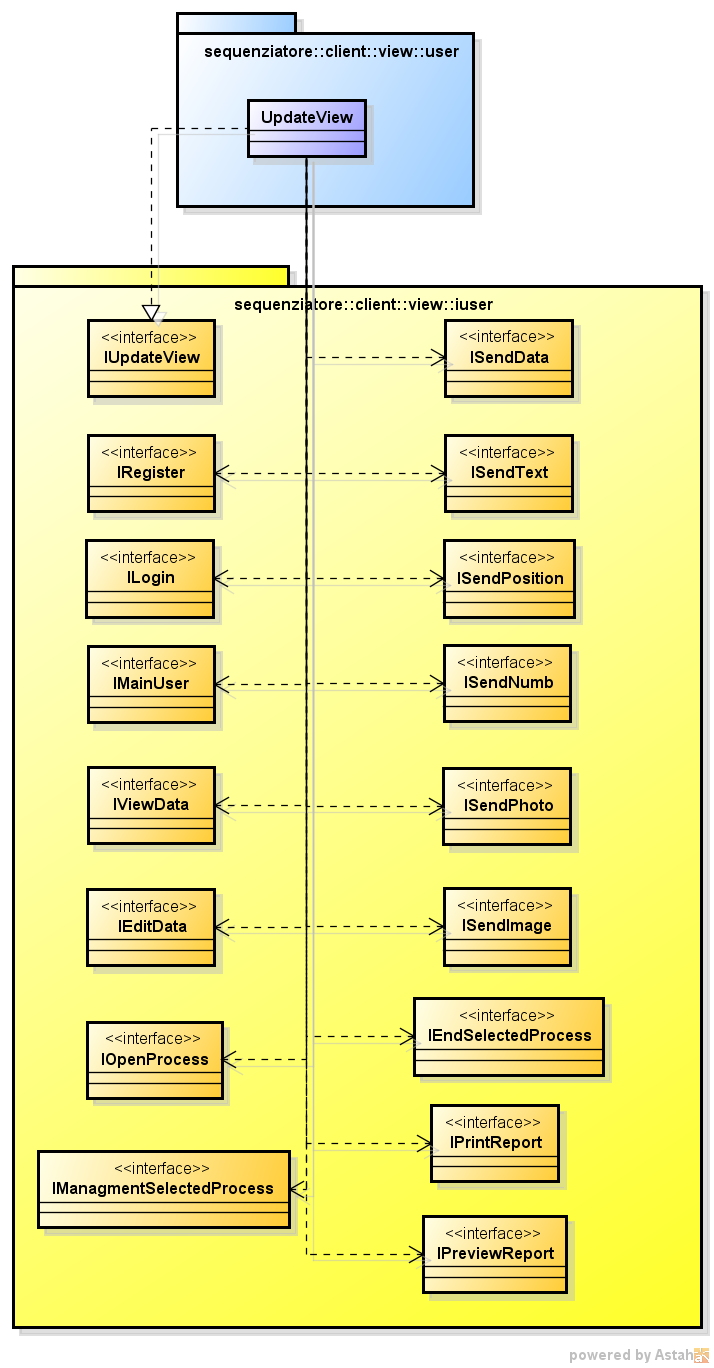
\includegraphics[scale=0.5]
{./pack/UpdateView.png} \caption{Diagramma relativo all'aggiornamento della view}
\end{figure}
\begin{itemize}
\item \textbf{Nome:} \texttt{IUpdateView};
\item \textbf{Package:} \texttt{\iViewUser{}};
\item \textbf{Descrizione:} Interfaccia che permette di gestire l’aggiornameno dei \textit{widget\ped{G}} della componente \textit{view};
\end{itemize}

\paragraph{ILogin}
\begin{itemize}
\item \textbf{Nome:} \texttt{ILogin};
\item \textbf{Package:} \texttt{\iViewUser{}};
\item \textbf{Descrizione:} Interfaccia che permette di gestire l'interfaccia grafica relativa alle richieste di autenticazione e chiusura della sessione da parte dell'utente.
\end{itemize}

\paragraph{IRegister}
\begin{itemize}
\item \textbf{Nome:} \texttt{IRegister};
\item \textbf{Package:} \texttt{\iViewUser{}};
\item \textbf{Descrizione:} Interfaccia che permette di gestire l'interfaccia grafica relativa alle richieste di registrazione da parte dell'utente.
\end{itemize}

\paragraph{IViewData}
\begin{itemize}
\item \textbf{Nome:} \texttt{IViewData};
\item \textbf{Package:} \texttt{\iViewUser{}};
\item \textbf{Descrizione:} Interfaccia che permette la realizzazione dei \textit{widget} per la visualizzazione dei dati dell'utente.
\end{itemize}

\paragraph{IEditData}
\begin{itemize}
\item \textbf{Nome:} \texttt{IEditData};
\item \textbf{Package:} \texttt{\iViewUser{}};
\item \textbf{Descrizione:} Interfaccia che permette la realizzazione dei \textit{widget} per la modifica dei dati personali dell'utente.
\end{itemize}

\paragraph{IChangePassword}
\begin{itemize}
\item \textbf{Nome:} \texttt{IChangePassword};
\item \textbf{Package:} \texttt{\iViewUser{}};
\item \textbf{Descrizione:} Interfaccia che permette la realizzazione dei \textit{widget} per la modifica della \textit{password} dell'utente.
\end{itemize}

\paragraph{IOpenProcess}
\begin{itemize}
\item \textbf{Nome:} \texttt{IOpenProcess};
\item \textbf{Package:} \texttt{\iViewUser{}};
\item \textbf{Descrizione:} Interfaccia che permette di realizzare i \textit{widget} per consentire la ricerca e la selezione di processi.
\end{itemize}

\paragraph{IManagementSelectedProcess}
\begin{figure}[H] \centering 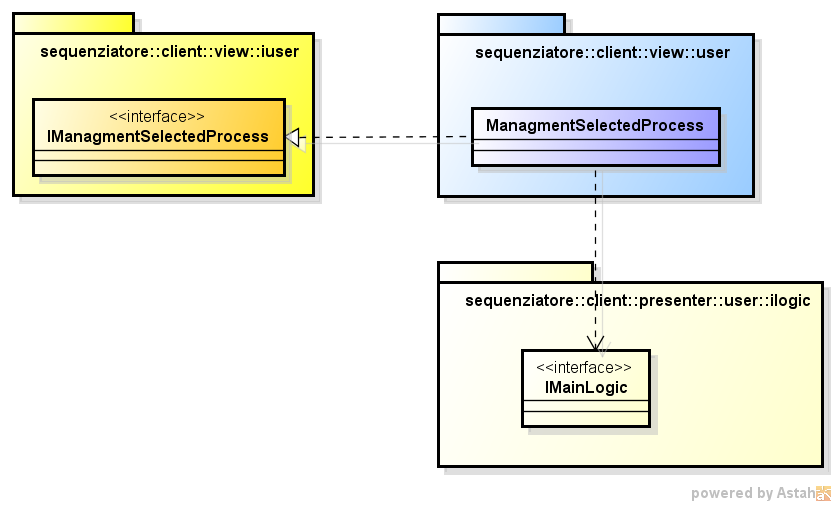
\includegraphics[width=%
\textwidth]
{./pack/ManagmentSelectedProcess.png} \caption{Diagramma gestione processo selezionato}
\end{figure}
\begin{itemize}
\item \textbf{Nome:} \texttt{IManagementSelectedProcess};
\item \textbf{Package:} \texttt{\iViewUser{}};
\item \textbf{Descrizione:} Interfaccia che permette di realizzare i \textit{widget} per visualizzare lo stato corrente del processo selezionato e i vincoli per concludere il passo.
\end{itemize}

\paragraph{ISendData}
\begin{figure}[H] \centering 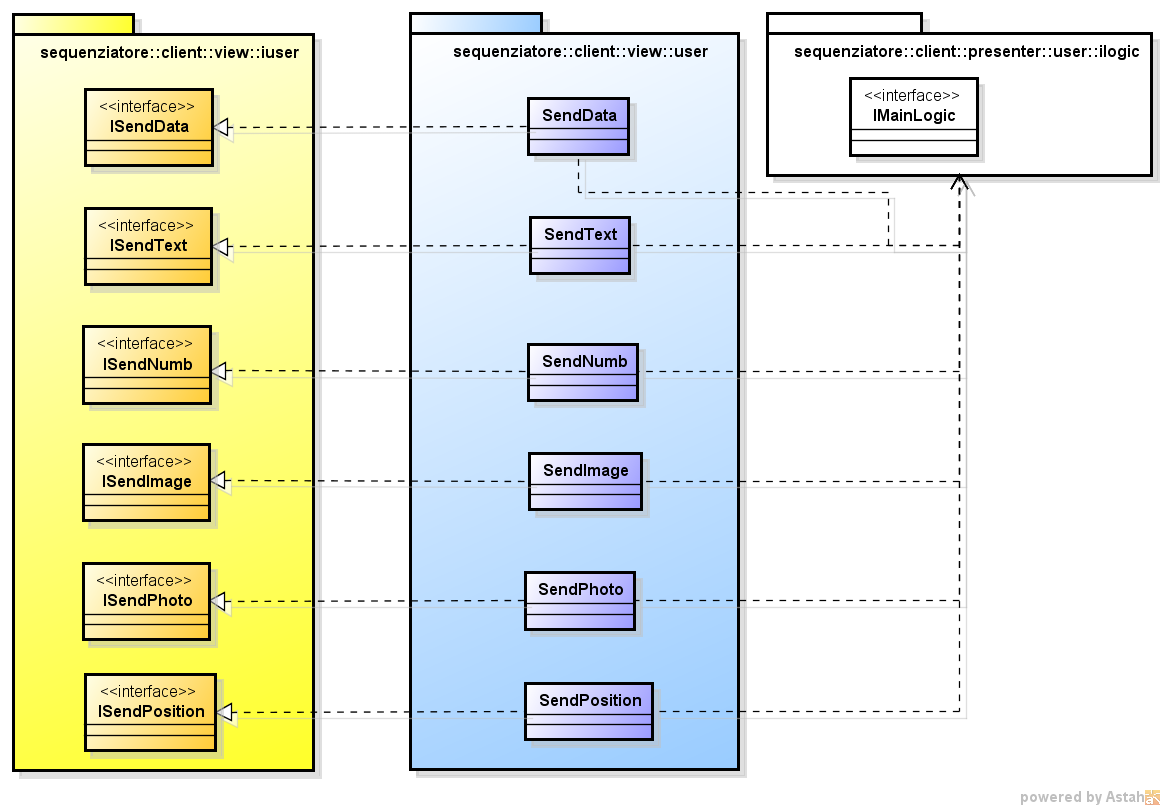
\includegraphics[width=%
\textwidth]
{./pack/SendData.png} \caption{Diagramma inserimento e invio dei dati}
\end{figure}
\begin{itemize}
\item \textbf{Nome:} \texttt{ISendData};
\item \textbf{Package:} \texttt{\iViewUser{}};
\item \textbf{Descrizione:} Interfaccia che permette di realizzare i \textit{widget} per inviare i dati richiesti per la conclusione del passo.
\end{itemize}

\paragraph{ISendText}
\begin{itemize}
\item \textbf{Nome:} \texttt{ISendData};
\item \textbf{Package:} \texttt{\iViewUser{}};
\item \textbf{Descrizione:} Interfaccia che permette di realizzare i \textit{widget} per inserire il testo da inviare per concludere il passo.
\end{itemize}

\paragraph{ISendNumb}
\begin{itemize}
\item \textbf{Nome:} \texttt{ISendNumb};
\item \textbf{Package:} \texttt{\iViewUser{}};
\item \textbf{Descrizione:} Interfaccia che permette di realizzare i \textit{widget} per inserire i dati numerici da inviare per concludere il passo.
\end{itemize}

\paragraph{ISendPosition}
\begin{itemize}
\item \textbf{Nome:} \texttt{ISendPosition};
\item \textbf{Package:} \texttt{\iViewUser{}};
\item \textbf{Descrizione:} Interfaccia che permette  di realizzare i \textit{widget} per inviare la posizione geografica per la conclusione di un passo. Inoltre consente di visualizzare eventuali messaggi d'errore nella rilevazione delle coordinate.
\end{itemize}

\paragraph{ISendImage}
\begin{itemize}
\item \textbf{Nome:} \texttt{ISendImage};
\item \textbf{Package:} \texttt{\iViewUser{}};
\item \textbf{Descrizione:} Interfaccia che permette di realizzare i \textit{widget} per inserire le immagini richieste per la conclusione del passo.
\end{itemize}

\paragraph{ISendPhoto}
\begin{itemize}
\item \textbf{Nome:} \texttt{ISendPhoto};
\item \textbf{Package:} \texttt{\iViewUser{}};
\item \textbf{Descrizione:} Interfaccia che permette di realizzare i \textit{widget} per consentire all'utente di scattare le fotografie richieste dal passo in esecuzione, e di inviarle.
\end{itemize}

\paragraph{IEndSelectedProcess}
\begin{figure}[H] \centering 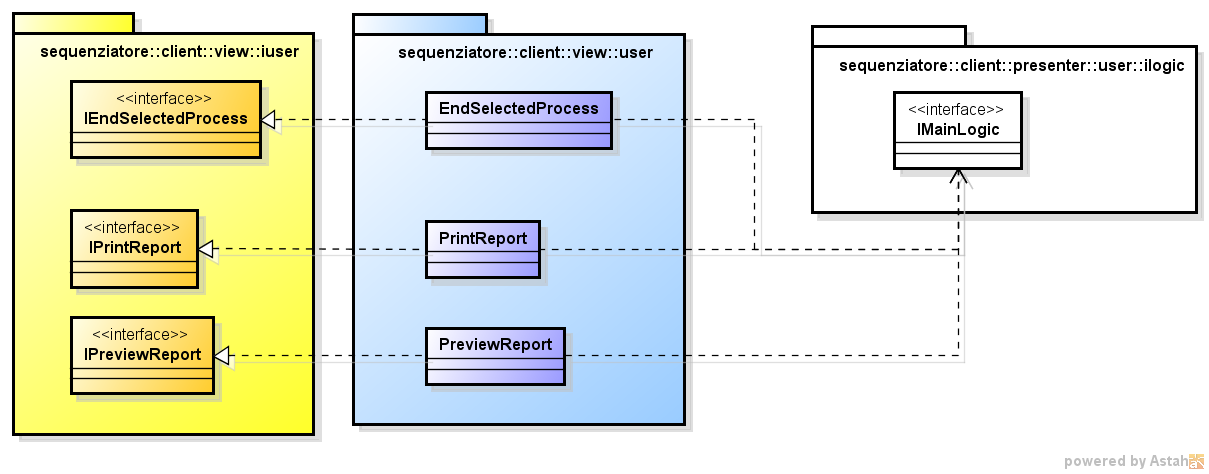
\includegraphics[width=%
\textwidth]
{./pack/EndSelectedProcess.png} \caption{Diagramma conclusione e stampa del rapporto}
\end{figure}
\begin{itemize}
\item \textbf{Nome:} \texttt{IEndSelectedProcess};
\item \textbf{Package:} \texttt{\iViewUser{}};
\item \textbf{Descrizione:} Interfaccia che permette di realizzare i \textit{widget} per visualizzare l'esito del processo e consentire le operazioni di conclusione del processo.
\end{itemize}

\paragraph{IPrintProcess}
\begin{itemize}
\item \textbf{Nome:} \texttt{IPrintProcess};
\item \textbf{Package:} \texttt{\iViewUser{}};
\item \textbf{Descrizione:} Interfaccia che permette di realizzare i \textit{widget} per consentire il salvataggio dei \textit{report} di fine processo.
\end{itemize}

\paragraph{IPreviewProcess}
\begin{itemize}
\item \textbf{Nome:} \texttt{IPreviewProcess};
\item \textbf{Package:} \texttt{\iViewUser{}};
\item \textbf{Descrizione:} Interfaccia che permette di realizzare i \textit{widget} per consentire la visualizzazione dei \textit{report} di fine processo.
\end{itemize}